\subsection{Neural Net Definitions}

Here we look into a neural network based on perceptron cells with an activation function.
A single perception can be regarded as a linear classifier, i.e. it is able to output
which of two linearly separable data sets a given point belongs to. In order to classify
more complex data sets, layers of perceptrons with non-linear activation functions are
required.

\begin{figure}[h] \centering 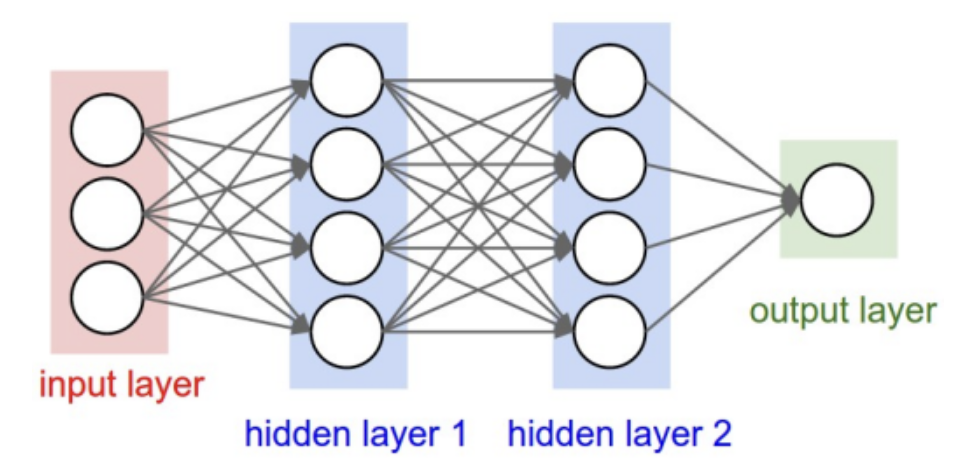
\includegraphics[width=0.75\textwidth]{neural_network}
    \caption{A fully connected multi-layer neural network with three inputs, two hidden
    layers, each with four perceptron nodes and an output layer with a single output node.
    (Source: \url{https://towardsdatascience.com})} \label{fig:neural_network}
\end{figure}

A neural net consists of $L$ layers with $n^l$ nodes in each layer $l=[0,L-1]$. For the
input layer $(l=0)$ the nodes are simple input nodes, while for the remaining layers
consist of perceptron nodes (see figure~\ref{fig:perceptron}). \\

A perceptron with an arbitrary activation function looks like this:
\begin{figure}[h] \centering 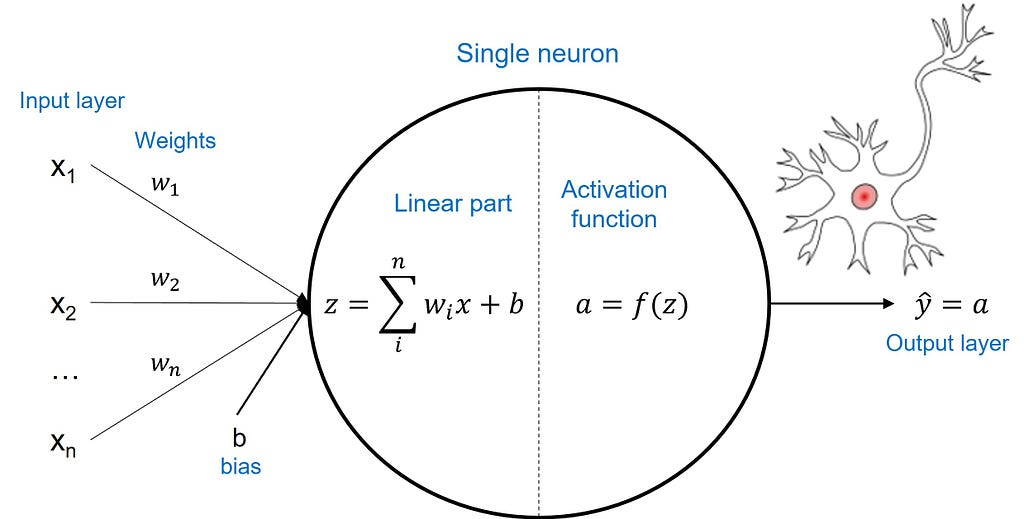
\includegraphics[width=0.75\textwidth]{single_neuron}
    \caption{A node of a neural network with inputs, bias and activiation function.
    (Source: \url{https://towardsai.net})}
    \label{fig:perceptron}
\end{figure}

\subsubsection*{Definitions:}
\begin{enumerate}
    \item We use a training dataset $X$ consisting of input-output pairs $(\vec{x}_i,
    \vec{y}_i)$, where $\vec{x}_i$ is the input and $\vec{y}_i$ is the desired or target
    output of the network on the input $\vec{x}_i$ ($\vec{y}_i$ is a label). The set of
    input-output training pairs of size $N$ is denoted $X = \{(\vec{x}_1,\vec{y}_1),
    \dots, (\vec{x}_N,\vec{y}_N)\}$.

    \item A neural network has learning parameters, weights and biases, that are
    collectivly denoted $\theta$. The nodes between different layers are fully connected,
    while there are no connections between nodes within the same layer. For
    backpropagation the parameters of primary interest are the weights $w^l_{tf}$,
    defining the weight\footnote{In this notation the index $t$ stands for \emph{to},
    whereas $f$ stands for \emph{from}. Index $t$ refers to nodes in layer $l$, while
    index $f$ refers to nodes in layer $l-1$ for the forward pass.} between the node with
    index $t$ in layer $l$ and the node with index $f$ in layer $l-1$, and $b^l_t$,
    defining the bias of the node with index $t$ in layer $l$. 

    \item A loss function $L(X,\theta)$, which defines a quantitative measure for the
    error between the desired output $\vec{y}_i$ and the calculated actual output
    $\vec{a}^l_i$ of the neural network on the input $\vec{x}_i$ for a given input pair
    $(\vec{x}_i, \vec{y}_i) \in X$ and a particular value of the learning parameters
    $\theta$.
\end{enumerate}

Following values are used to define the network:
\begin{itemize}
    \item $x_t$, the input at index $t$ of an input vector $\vec{x}_i$ of the training set
    in the input layer ($x_t = a^{l=0}_t$ after activation of the input layer in the
    implementation, see below for definition of $a^l_t$).

    \item $w^l_{tf}$, the weight between the node with index $t$ (\emph{\underline{t}o})
    in layer $l$ and the node with index $f$ (\emph{\underline{f}rom}) in layer $l-1$.

    \item $b^l_t$, the bias of the node with index $t$ in layer $l$.
    
    \item $z^l_t = \sum_{f}{w^l_{tf} a^{l-1}_f} + b^l_t$ is the total input the node gets
    from the activated nodes of the previous layer and it's bias.
    
    \item Activation functions $f_h$ for the \underline{h}idden layers and the
    \underline{o}utput layer $f_o$.
    
    \item The activation $a^l_t$ at index $t$ in layer $l$: $a^l_t = f_h(z^l_t)$ in hidden
    layers or $a^{L-1}_t = f_o(z^{L-1}_t)$ for the output layer. The activation function
    for the input layer is the identity function in the implementation.

    \item $a^{L-1}_t$ is the output component at the index $t$ in the output layer at the
    given input $\vec{x}_i$. The intended output is defined by $\vec{y}_i$ as second part
    of the training pair $(\vec{x}_i, \vec{y}_i)$, where $y_t$ is the component $t$ of
    $\vec{y}_i$.
\end{itemize}

The goal of training is to minimize the loss function and thus to minimize the remaining
error for a given set of training data.  A typical example of a loss function is the
quadratic cost function (Mean Squared Error (MSE) with additional factor of $\frac{1}{2}$
for easy calculation of its derivative). The total loss is an average of the $N$ partial
losses $L_i$ for each training pair $(\vec{x}_i, \vec{y}_i)$ as shown in
equation~(\ref{eq:mse_loss_func}), where the partial loss itself is a sum over the
contributions of each component $t$ of the difference between the actual output vector of
the network $\vec{a}^{L-1}_i$ and the intended output vector $\vec{y}_i$ for a given
training pair $i$.

\begin{equation}
    L(X,\theta) = \frac{1}{N}
    \sum_{i=1}^{N}{\frac{1}{2}\lVert \vec{a}^{L-1}_i - \vec{y}_i \rVert^2}
    = \frac{1}{N} \sum_{i=1}^{N}{\underbrace{\sum_{t}{\frac{1}{2} (a^{L-1}_t - y_t)^2}}_{L_i}}
    \label{eq:mse_loss_func}
\end{equation}

We need to understand how the deviation of the actual output to the desired output depends
on the choice of learning parameters $\theta$, i.e. the weights $w$ and the bias values
$b$. In order to minimize the loss function, and thus the deviation between actual and
desired output, gradient descent is used. This means that the training parameters have to
be changed in a direction against the gradient of the function $L$. This requires to
calculate all partial derivatives of the loss function with respect to the weights
$\pd{L}{w}$ and to the biases $\pd{L}{b}$ in order to update them with $\eta$ as learn
rate according to
\begin{subequations}
    \begin{align}
    w^{new} & =  w^{old} - \eta \pd{L}{w}
    \label{eq:update_weights} \\
    b^{new} & =  b^{old} - \eta \pd{L}{b}
    \label{eq:update_bias}
\end{align}
\end{subequations}

To understand why this is the case, let's consider an arbitrary cost function with three
parameters $C(w_1,w_2,b)$ as an example. For small changes we get:
\begin{equation}
    \Delta C \approx \pd{C}{w_1}\Delta w_1 + \pd{C}{w_2}\Delta w_2 +\pd{C}{b}\Delta b
\end{equation}
So $\Delta C \approx \vec{\nabla} C \cdot \Delta \vec{v}$ with $\vec{\nabla} C =
(\pd{C}{w_1}, \pd{C}{w_2}, \pd{C}{b})^T$ and $\Delta \vec{v} = (\Delta w_1, \Delta w_2,
\Delta b)^T$.\\

To minimize C, we need to assure that $\Delta C < 0$. \\

If we specifically choose $\Delta \vec{v} = -\eta \vec{\nabla} C$, i.e. select the change
of $\Delta \vec{v}$ against the direction of the gradient vector, we get
\begin{equation}
    \Delta C \approx \vec{\nabla} C \cdot (-\eta \vec{\nabla} C)
    = -\eta \vec{\nabla} C \cdot \vec{\nabla} C
    = -\eta \lVert \vec{\nabla} C \rVert ^2
\end{equation}
which assures a negative $\Delta C$, because $\lVert \vec{\nabla} C \rVert ^2$ is a
positive value. \\

In practise we can either calculate the gradient for the full training set, or rather
approximate the gradient by selecting a random subset of the training samples (called a
mini-batch), or directly calculate the gradient we get for each individual training sample
pair (called stochastic gradient descent). The resulting gradient is applied according
to equations~(\ref{eq:update_weights}) and (\ref{eq:update_bias}) to update the weights
and biases. The approaches of gradient approximation are mainly used to reduce the
computational effort. \\

It is called an epoch, when the neural net has seen all available training data once
during a training cycle. The training typically covers several hundred epochs for
minimizing the loss function. \\

The available data is normally split into training data, validation data, test data in a
ratio of 70:20:10. The training data set is used to learn the training parameters. The
validation data is used for initially optimizing the meta parameters (e.g. learning rate,
batch sizes, activation functions, etc.). The test data set is used to calculate the
quality of the training as a result (precision, recall, accuracy). All subsets must of
course be large enough to be representative for the full available data set or we run into
trouble due to biased data in the subsets. \\

The learning or training cylce for a neural network looks like this:
\begin{figure}[h] \centering 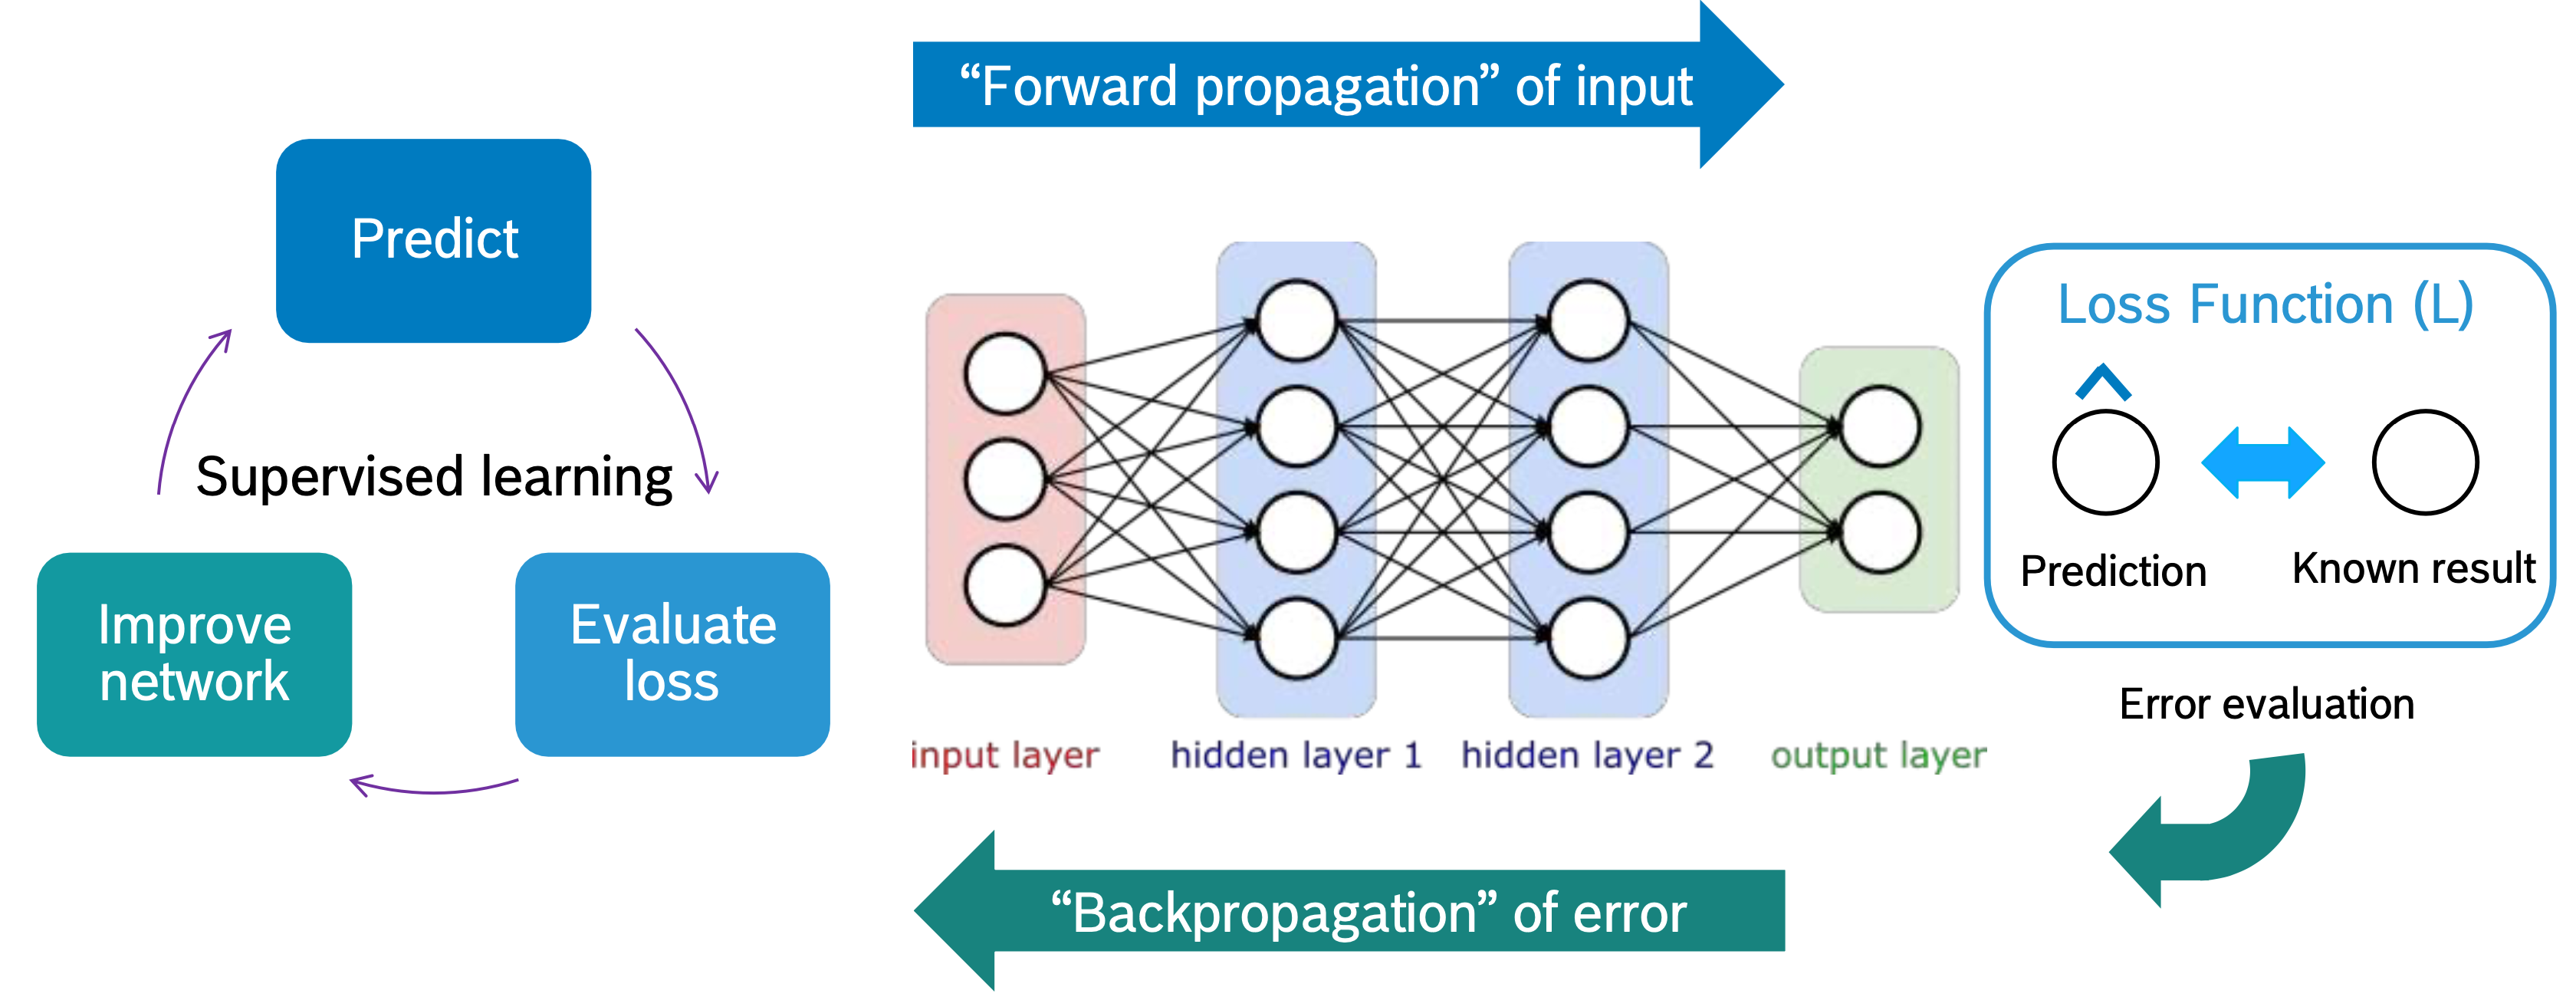
\includegraphics[width=0.75\textwidth]{nn_learning_cycle}
    \caption{Training or learning cycle of a neural network.
    (Source: Bosch AIMEX training)}
    \label{fig:training_cycle}
\end{figure}

TODO: \emph{fill in prodedure to compute accuracy, precision, etc. here}

\newpage
